%! Author = adnansiddiquei
%! Date = 19/03/2024

\section{Q2 - Planet detection and characterisation via RVs}\label{sec:q2}
\subsection{Initial Exploration}\label{subsec:q2-init-exploration}
Radial velocity measurements are extremely useful for detecting exoplanets and characterising their properties.
These measurements are taken by observing the Doppler shift in the spectrum of a star, indicating a shift in the star's velocity
tangential to the observer's line of sight.
However, a variety of stellar "nuisance" signals can also induce these shifts in the star's spectrum.
These include things like oscillations and granulations which occur over the timescales of minutes to hours; rotationally-modulated
activity which occur over the timescale of days to weeks, often in line with the star's rotation period; and magnetic cycles
which are long-term variations in the star's magnetic field.
Likewise, not all periodic signals in the RV data will be due to RV data or stellar signals, it is important to note
that instrument noise or poor sampling (aliasing) can also induce periodic signals in the RV data.

The radial velocity is extracted from an observed spectrum using a cross-correlation function (CCF) which compares the observed
spectrum to a template spectrum of what the star should look like at rest.
From this CCF, two stellar activity indicators can also be extracted: the full width at half maximum (FWHM) and the bisector
span (BIS).
These indicators correlate to the stellar activity signals mentioned above, and can be used to filter out the stellar
activity signals from the radial velocity measurements.

\begin{table}[htb]
    \centering
    \begin{tabular}{ccc}
        \toprule
        \toprule
        Parameter & Units & Value \\
        \midrule
        Rotation Period $P_{rot}$ & days & $31 \pm 10$ \\
        \addlinespace
        Mass $M_{\star}$ & $M_{\odot}$ & $0.69 \pm 0.01$ \\
        \addlinespace
        Effective Stellar Temp. $T_{eff}$ & K & 4500 \\
        \bottomrule
    \end{tabular}
    \caption{Properties of star CB 01223.}
    \label{tab:star_props}
\end{table}

\begin{figure}[htb]
    \centering
    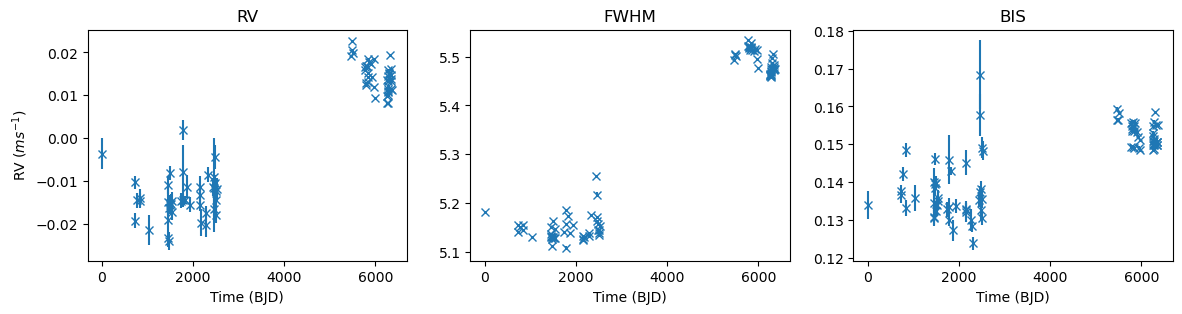
\includegraphics[width=1\textwidth]{figures/data_plot}
    \caption{The radial velocity, FWHM and BIS data for star CB 01223.}
    \label{fig:data_plot}
\end{figure}

Table~\eqref{tab:star_props} shows the properties of the star CB 01223 that this section will analyse and characterise.
Figure~\eqref{fig:data_plot} shows a plot of the RV, FWHM and BIS data for this star.
Initial qualitative inspection of the RV, FWHM and BIS shows a long term correlated positive trend, where all three of the
datasets show a jump in the RV between the two groups of measurements (centered around 2000 BJD and 6000 BJD).
Given the correlation, this indicates that there is a likely long term stellar activity signal present in the data, and given
the time scale, it is likely due to the star's magnetic cycle.

\begin{figure}[htb]
    \centering
    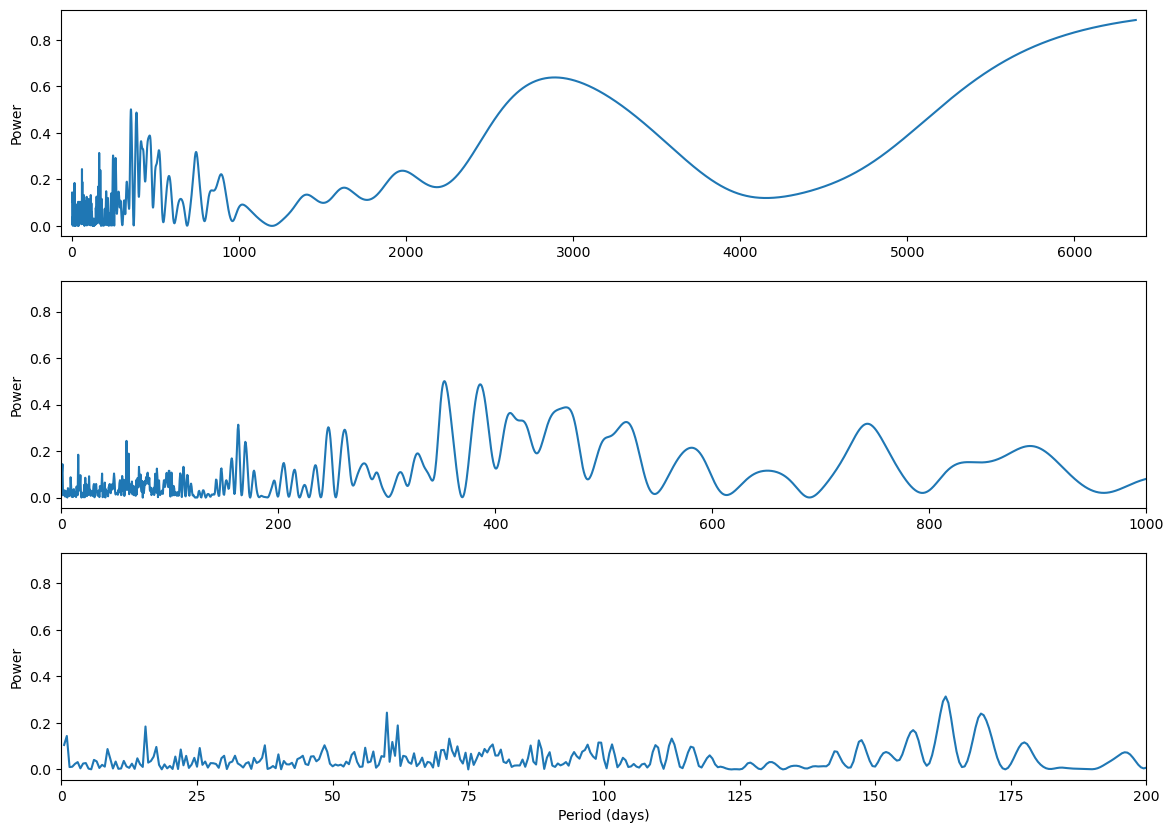
\includegraphics[width=1\textwidth]{figures/lombscargle_periodogram_q2}
    \caption{Lombscargle periodogram of the RV data for star CB 01223. The periodograms are shown at 3 different period
    ranges, with the top plot showing the full range of periods, and the bottom two plots showing zoomed in views of the
    periodogram.}
    \label{fig:lombscargle_periodogram_q2}
\end{figure}

An initial LombScargle periodogram~\cite{lomb, scargle} as shown in Figure~\eqref{fig:lombscargle_periodogram_q2} yields
little useful information.
A peak near the 3000-day mark is likely due to the 2 groups of measurements, and the zoomed in views show no significant
peaks worth exploring.

\subsection{Quantitative Analysis - Evidence of Exoplanets?}\label{subsec:q2-quantitative-analysis}
The exoplanet search conducted in this report follows closely with the methodology used by Faria, et al. (2022)~\cite{faria2022}
to search for exoplanets in the radial velocity data of Proxima Centauri.
They initially utilised a joint RV and FWHM Gaussian process (GP) model to model the stellar activity signals in the data,
and subtracted this from the RV data before fitting a Keplerian model to the residuals.
This methodology is extended slightly and a joint GP model is fit to all three of the RV, FWHM and BIS datasets to model
the stellar activity.

\begin{equation}\label{eq:qp-kernel}
    \mathcal{K}_{\text{QP}}(\tau) =
    \theta_1^2 \exp
    \left[
        -\frac{\tau^2}{2 \theta_2^2} - \frac{\sin^2 \left( \frac{\pi |t_{i} - t_{j}|}{\theta_3} \right)}{\theta_4^2}
    \right]
\end{equation}

Equation \eqref{eq:qp-kernel} shows the Quasi-Periodic (QP) kernel used in the GP model, where all $\theta_{2}, \theta_{3}
\theta_{4}$ were all shared between the RV, FWHM and BIS datasets (hence the joint GP model), but $\theta_{1}$ was allowed
to float for each dataset.

\begin{table}[htb]
    \centering
    \begin{tabular}{ccc}
        \toprule
        \toprule
        Parameter & Units & Prior \\
        \midrule
        Amplitude $\theta_{1}$ RV & $ms^{-1}$ & $\mathcal{U}(1e^{-4}, 3 \Delta$RV$)$ \\
        \addlinespace
        Amplitude $\theta_{1}$ FWHM & $ms^{-1}$ & $\mathcal{U}(1e^{-4}, 3 \Delta$FWHM$)$  \\
        \addlinespace
        Amplitude $\theta_{1}$ BIS & $ms^{-1}$ & $\mathcal{U}(1e^{-4}, 10 \Delta$BIS$)$ \\
        \addlinespace
        Exp Length Scale $\theta_{2}$ & $s$ & $\mathcal{U}(1e^{-4}, 3 \Delta$t$)$ \\
        \addlinespace
        Stellar Period $\theta_{3}$ & $s$ & $\mathcal{G}(31, 10)$ \\
        \addlinespace
        Periodic Length Scale $\theta_{4}$ & $s$ & $\mathcal{U}(1e^{-4}, 3 \Delta$t$)$ \\
        \addlinespace
        Jitter $j$ & $ms^{-1}$ & $\mathcal{LU}(1e^{-10}, 1e^{-6})$ \\
        \bottomrule
    \end{tabular}
    \caption{Parameters and priors for the joint QP GP model on the RV, FWHM and BIS datasets.
    $\mathcal{U}(a, b)$ denotes a uniform prior between $a$ and $b$; $\mathcal{G}(\mu, \sigma)$ denotes a Gaussian prior
    with mean $\mu$ and standard deviation $\sigma$; and $\mathcal{LU}(a, b)$ denotes a log-uniform prior between $a$ and $b$.}
    \label{tab:stellar_gp_priors}
\end{table}

Table~\eqref{tab:stellar_gp_priors} shows a list of all the parameters and priors used for the joint stellar activity
GP model.
Note that the data was standardised before fitting the GP model to help with convergence, the table lists the priors
in the non-standardised scale, but these were converted to the standardised scale before fitting.
Bringing the data to a common scale also allowed for a single jitter term to be used across all three datasets, reducing
the number of parameters that needed to be fit.
The jitter term was given a log-uniform prior to allow for a wide range of values, but the upper limit was set to $1e^{-6}$
In general, relatively uninformative priors were used for all the remaining parameters, all priors covered a multiple of the entire
extent of their respective data.
The only exception was the stellar period $\theta_{3}$ which was given a Gaussian prior centered around the rotation
period derived from the TESS photometry measurements.

A Markov Chain Monte Carlo (MCMC) simulation was then run, drawing initial samples from these priors with 250 walkers and
2000 iterations per walker.
Samples were extracted with a burn in of 100 iterations and a thinning factor of 20 to reduce autocorrelation.
Figure~\eqref{fig:stellar_noise_corner_plot} shows the corner plot of this MCMC simulation, and
Figure~\eqref{fig:stellar_noise_fit} shows the GP model fit to the RV, FWHM and BIS datasets from the maximum likelihood
sample of the MCMC simulation.
The MCMC simulation found 2 distinct distributions for the stellar period $\theta_{3}$ in the posterior space, as shown
in Figure~\eqref{fig:stellar_period_2dhist} which plots a 2D histogram of the stellar period $\theta_{3}$ and the log-likelihood
of the MCMC samples, illustrating the two distinct distributions.
The maximum likelihood sample of the MCMC simulation has a period of 35.3 days.

\begin{figure}[htb]
    \centering
    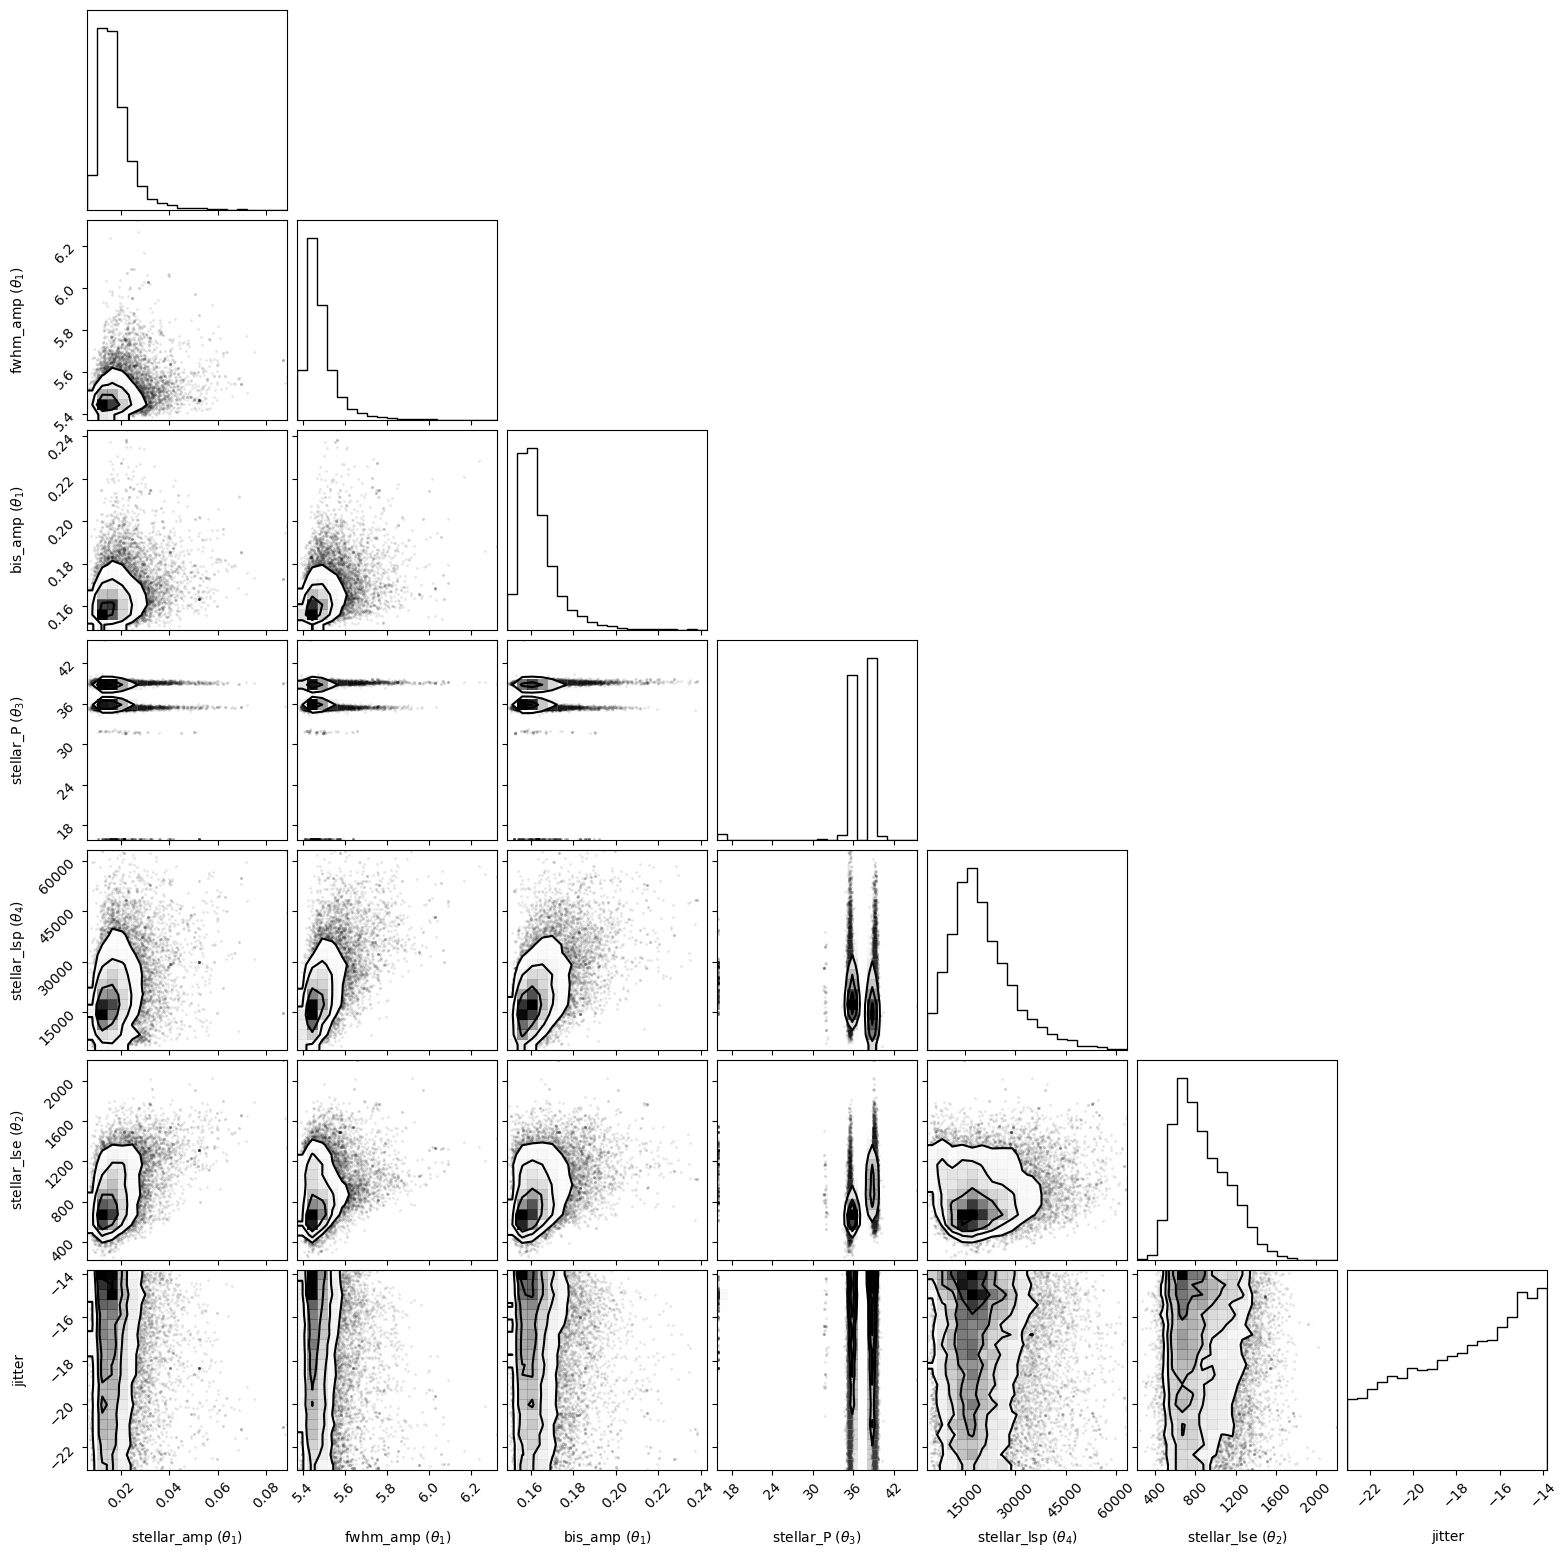
\includegraphics[width=1\textwidth]{figures/stellar_noise_corner_plot}
    \caption{A corner plot of the MCMC simulation for the joint QP GP model on the RV, FWHM and BIS datasets.
    The bottom 10th percentile of the samples (based on the log-likelihood) were dropped to remove the tails of the distributions,
    for better visualisation.}
    \label{fig:stellar_noise_corner_plot}
\end{figure}

\begin{figure}[htb]
    \centering
    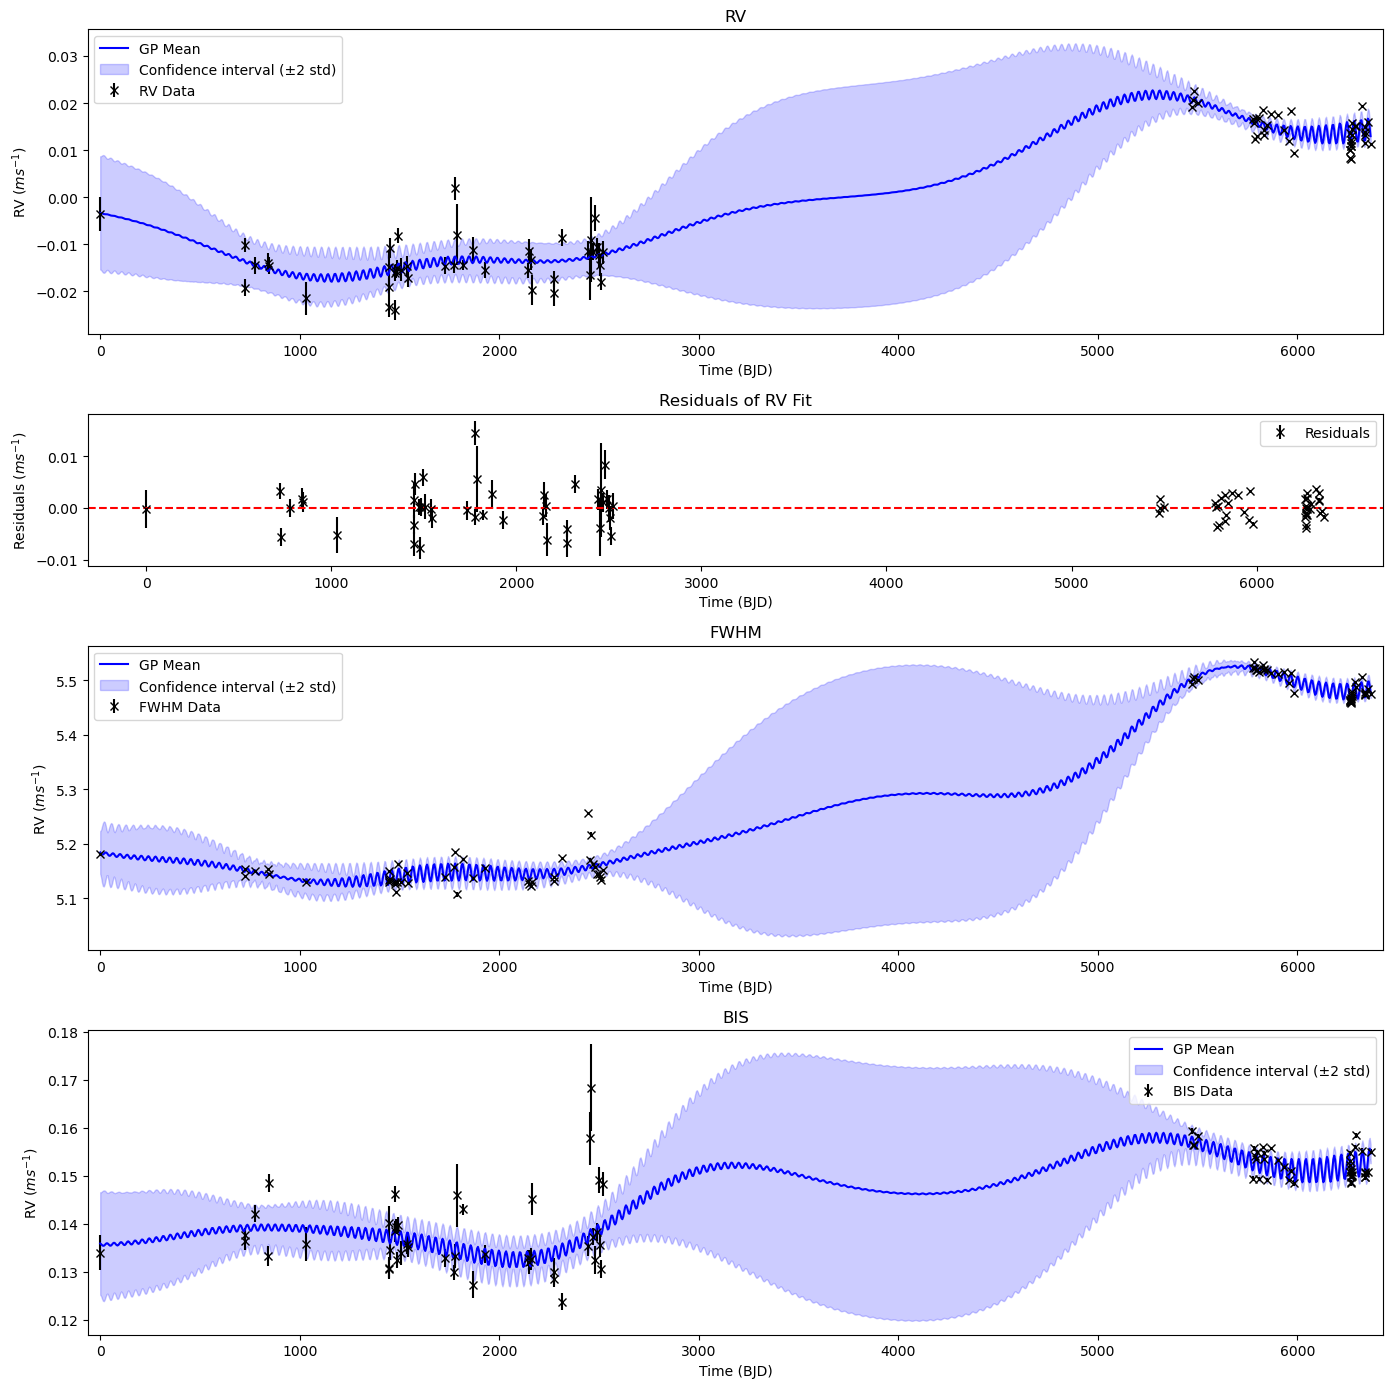
\includegraphics[width=1\textwidth]{figures/stellar_noise_fit}
    \caption{The GP model fit to the RV, FWHM and BIS datasets for star CB 01223.
    The fitted GP uses the parameters from the maximum likelihood sample of the MCMC simulation.
    The second plot shows the residuals of the GP model fit to the RV data.}
    \label{fig:stellar_noise_fit}
\end{figure}

\begin{figure}[htb]
    \centering
    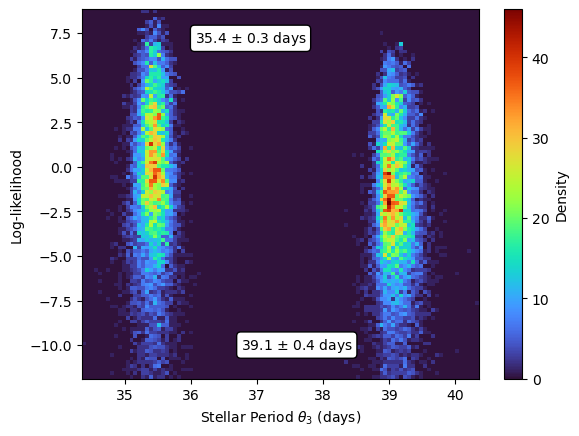
\includegraphics[width=0.8\textwidth]{figures/stellar_period_2dhist}
    \caption{The joint distribution of the stellar period $\theta_{3}$ and log-likelihood of the MCMC samples.
    The text boxes show the mean and standard deviation of the stellar period $\theta_{3}$ for each of the two distributions.}
    \label{fig:stellar_period_2dhist}
\end{figure}

As per the methodology used by Faria, et al. (2022)~\cite{faria2022}, the GP model was subtracted from the RV data as shown
in the residual plot in Figure~\eqref{fig:stellar_noise_fit}.
A simplified Keplerian model, in the form of a sine wave was then fit to the residuals to identify any potential exoplanets.
The single planet model consisted of 3 parameters: the semi-amplitude $K$, the orbital period $P$ and the phase $\phi$,
likewise, the 2 planet model consisted of 6 parameters: the semi-amplitudes $K_{1}, K_{2}$, the orbital periods $P_{1}, P_{2}$
and the phases $\phi_{1}, \phi_{2}$.
Both of these models used the priors shown in Table~\eqref{tab:kepler_priors}, the priors were chosen to be relatively
uninformative, covering at least the entire range of values that the parameters could take.

\begin{table}[htb]
    \centering
    \begin{tabular}{ccc}
        \toprule
        \toprule
        Parameter & Units & Prior \\
        \midrule
        Semi-amplitude $K$ & $ms^{-1}$ & $\mathcal{U}(0, 1.5 \Delta$Residuals$)$ \\
        \addlinespace
        Orbital Period $P$ & $s$ & $\mathcal{U}(0, 3 \Delta$t$)$  \\
        \addlinespace
        Phase Offset $\phi$ & $s$ & $\mathcal{U}(0, 2\pi)$ \\
        \bottomrule
    \end{tabular}
    \caption{Parameters and priors for the joint QP GP model on the RV, FWHM and BIS datasets.
    Both of the single and 2 planet models used these same priors.}
    \label{tab:kepler_priors}
\end{table}

The MCMC simulation was run in a nested manner by running a simulation, and then shrinking the uniform prior on the orbital
period $P$, with the new prior being informed by the posterior distribution of the previous simulation.
This was done to ensure that no bias was added into the priors initially, but to also allow the MCMC simulation to sequentially
explore the higher likelihood regions of the posterior space to yield a better final estimate of the parameters.

For the single planet model, the initial MCMC simulation found that the top 5th percentile of the samples (based on the
log-likelihood) has a period in the range $[1.72, 53.10]$, and so a second simulation was conducted with a new uniform
prior on the orbital period $P$ being $\mathcal{U}(0, 58)$.
This yielded a best fit model as shown in Figure~\eqref{fig:1planet_model_fit}, with the corner plot of the simulation
samples given in Figure~\eqref{fig:1planet_model_corner_plot}.
Figure~\eqref{fig:1planet_model_fit} also shows the posterior distribution of the orbital period $P$ and semi-amplitude $K$.
The best fit model had a period of $5.09 \pm 0.87$ days and a semi-amplitude of $2.24e^{-3} \pm 0.61e^{-3} ms^{-1}$.
The best fit model was taken as the maximum likelihood sample of the MCMC simulation, and the errors were given
as 2 sigma on the posterior distributions, to indicate a 95\% confidence region.
As evident on the corner plot in Figure~\eqref{fig:1planet_model_corner_plot}, there were several peaks in the posterior
distribution of the orbital period $P$ in multiples of roughly 5 days (which is to be expected), and as such, the
errors on the orbital period $P$ was calculated using only the samples centered around 5.09 days.

Similar exploration on the 2 planet model did not yield any significant results indicating the possibility of a second
exoplanet and as such, the single planet model was taken as the best fit model to the RV data for star CB 01223.

Table \eqref{tab:final_posteriors} shows a summary of the final posterior distributions for all key parameters and derived
properties for star CB 01223 in the single planet model.
The planet was computed to have a semi-major axis of $0.051 \pm 0.020$ AU, indicating that it lives very close to the host star,
making it likely to be a hot Jupiter.

\begin{figure}[htb]
    \centering
    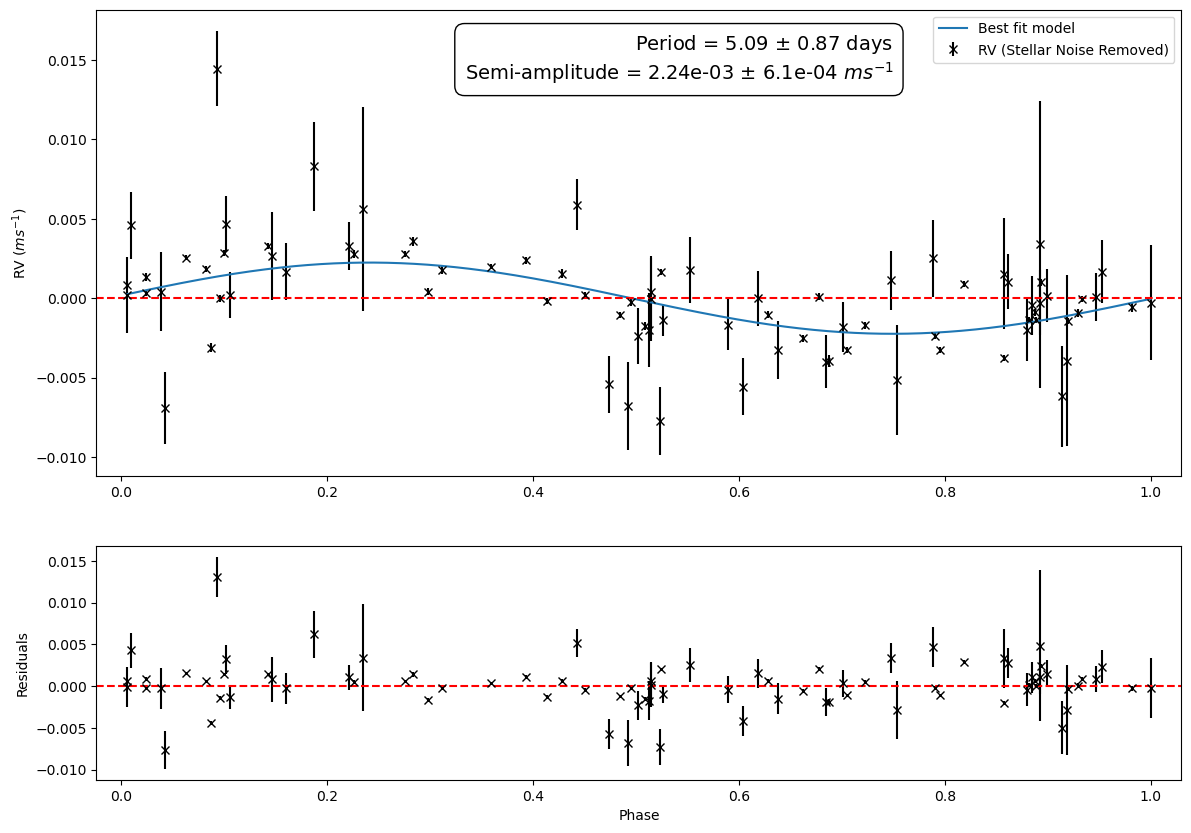
\includegraphics[width=0.8\textwidth]{figures/1planet_model_fit}
    \caption{The best fit single planet model to the RV data for star CB 01223.
    The posterior distribution of the orbital period $P$ and semi-amplitude $K$ are shown in the top right corner of the plot,
    the errors given are 2 sigma errors on the parameters.}
    \label{fig:1planet_model_fit}
\end{figure}

\begin{figure}[htb]
    \centering
    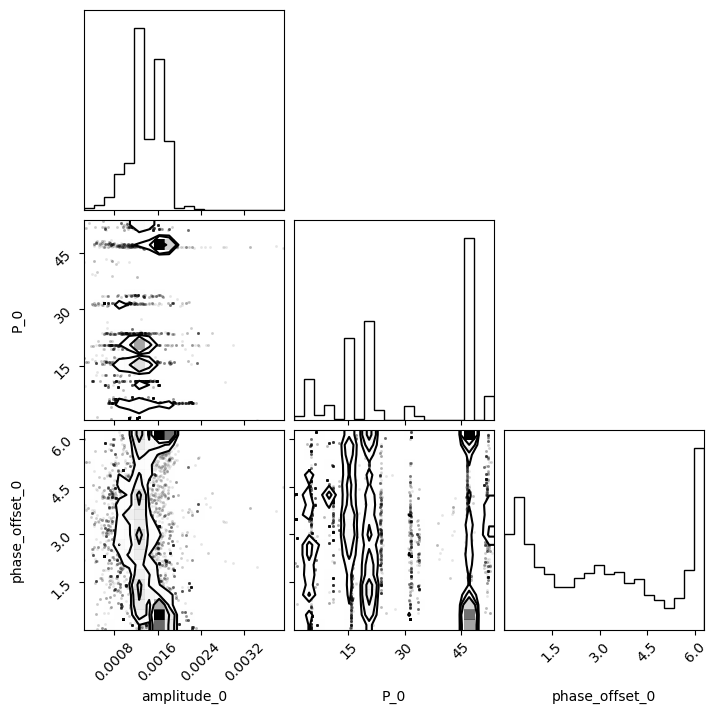
\includegraphics[width=0.8\textwidth]{figures/1planet_model_corner_plot}
    \caption{A corner plot of the MCMC simulation for the single planet model on the RV data.}
    \label{fig:1planet_model_corner_plot}
\end{figure}

\begin{table}[htb]
    \centering
    \begin{tabular}{ccc}
        \toprule
        \toprule
        Parameter & Units & Prior \\
        \midrule
        Stellar Period $P_{\star}$ & $days$ & $35.4 \pm 0.3$ \\
        \addlinespace
        Planet Orbital Period $P_{planet}$ & $days$ & $5.09 \pm 0.87$  \\
        \addlinespace
        Planet Semi-amplitude $K$ & $ms^{-1}$ & $2.24e^{-3} \pm 0.61e^{-3}$ \\
        \addlinespace
        Planet Semi-major Axis $a$ & $AU$ & $0.051 \pm 0.020$ \\
        \bottomrule
    \end{tabular}
    \caption{Final summary of posterior distributions for all key parameters and derived properties for star CB 01223
    in the single planet model. All errors are quoted as 2 sigma errors, to indicate a 95\% confidence region.}
    \label{tab:final_posteriors}
\end{table}
